\section{Precios}

Para el análisis de los precios se cuenta con un poco más de 1.5 millones de registros, que indican el precio de cada producto e información de contexto. Por medio de otros set de datos, como ser el que tiene los datos de las sucursales y detalles de los productos es que se harán análisis particulares en secciones próximas, pero en este caso el análisis estará apuntado al análisis de los precios en soledad.
Lo primero que se busca es por medio de un histograma conocer como es la distribución de los precios, como objetivo se busca entender si los mismos siguen alguna distribución o patrón.

\begin{figure}[h]
\centering
\fbox{
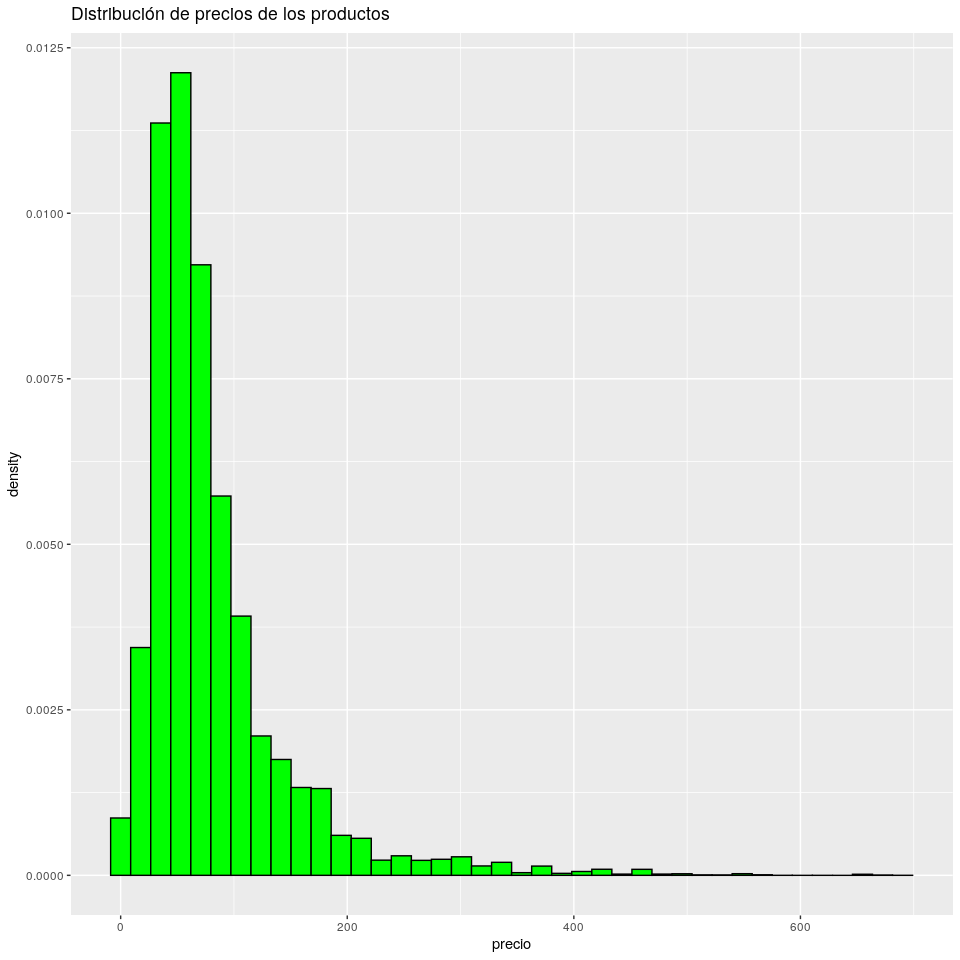
\includegraphics[width=0.8\textwidth]{img/histograma_precios_productos.png}
}%
\caption{Histograma precios}
\label{histograma}
\end{figure}


En cuanto al histograma de la figura \ref{histograma}, se puede evidenciar claramente una asimetría a derecha y como primer aproximación se puede ver como la mayoría de las mediciones marcan valores cercanos a los 80 Pesos.\\
Se visualiza en la siguiente tabla los valores significativos de todos los precios.\\

\begin{center}
 \begin{tabular}{||l c c c c c||} 
 \hline
 Minimo & 1st Qu & Mediana & Promedio & 3rd Qu & Máximo \\ [0.5ex] 
 \hline\hline
 2.85 & 42.00 & 62.90 & 80.79 & 95.99 & 693.00 \\ 
 \hline
 \hline
\end{tabular}
\end{center}

En principio el valor máximo y mínimo observado podrían indicar la presencia de valores anómalos o outliers en las mediciones, sobre todo teniendo en cuenta que el valor de mediana y Promedio es del orden de magnitud diferente a los dos extremos.


\subsection{Datos Atípicos}

Interesa conocer si la presencia de datos atípicos dentro de las mediciones de precios, estos podrían seguir dos naturalezas de origen:

\begin{enumerate}
    \item Datos mal cargados u originados con algún defecto en su medición.
    \item Precios que se corresponden con productos, pero que dependiendo de la cantidad de casos y de su naturaleza quizás no tenga sentidos mantenerlos en el análisis.
\end{enumerate}


Se generara un primer boxPlot para entender gráficamente como es la distribución de los precios para encontrar datos atípicos y poder catalogarlos para luego analizar si es necesario quitarlos o dejarlos entre los datos a estudiar.

\begin{figure}[h]
\centering
\fbox{
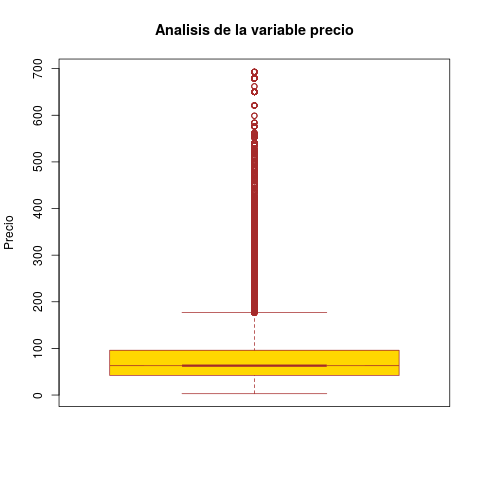
\includegraphics[width=0.65\textwidth]{img/boxplot_basico.png}
}%
\caption{Precios}
\label{boxplot}
\end{figure}




En la figura \ref{boxplot} de observa que los datos que pueden considerarse outliers son aquellos precios con un valor mayor a \$200,00. \\
Se puede evidenciar que hay gran cantidad de datos por sobre el bigote superior, con lo cual se ensayaron algunas técnicas para exploración de estos datos, para entender si eran o no datos atípicos.\\
En un primer momento se realizó el mismo BoxPlot pero eliminando toda medición ubicada a 1,5 veces la distancia inercuartil por arriba y por abajo, como resultado se obtuvo un diagrama muy similar al anterior donde la diferencia radicaba en que los outliers se empezaban a producir del mismo modo a partir de los \$150 con lo cual no significo en ninguna mejora para el análisis.\\
En segundo lugar se propuso eliminar un porcentaje de datos en las puntas superiores e inferiores pero nuevamente no mostraron resultados concluyentes.\\
Fue por ello y debido a que la mayor cantidad de datos atípicos se mostraban en las bandas más altas de precios que se decidido realizar un análisis de BoxPlot pero con los valores superiores a \$290 para entender como era la distribución de esos valores altos en más detalle.


\begin{figure}[h]
\centering
\fbox{
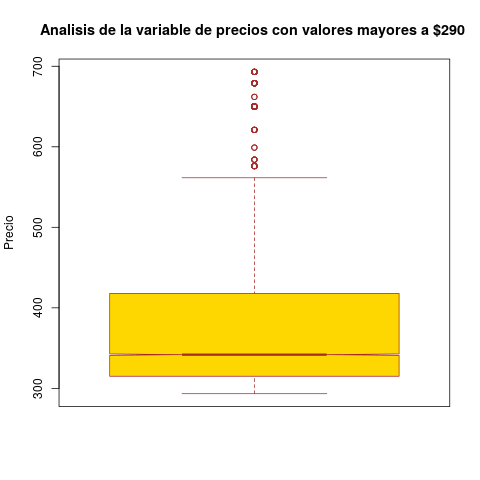
\includegraphics[width=0.65\textwidth]{img/boxplot_mayor290.png}
}%
\caption{Precios mayores a 290}
\label{boxplot_mayor290}
\end{figure}


Se aprecia que existen muy pocas observaciones ahora por encima del bigote superior, figura \ref{boxplot_mayor290}, por lo que se llevo a cabo una investigación de estas mediciones una a una para entender cual era el origen de las mismas.\\
Lo que se encontró en estos casos, es que estas mediciones se correspondían con precios correctamente medidos pero sobre productos de alto valor como ser una bebida importada (Whiskey) o similar, no representando un error en la medición ni tampoco un conjunto de datos completamente aislados, sino pequeños grupos que representan un producto en particular y que en todas sus mediciones se comportan de manera similar.\\
Es por ello que, como existen desigualdades entre los precios, se decide no eliminar partes ni recortar el set original de datos.







\section{Barrios Porteños}

Ya que se contaba con el dato de latitud y longitud donde cada punto de venta estaba ubicado, se comenzó el análisis de los datos haciendo un mapeo entre la posición geoespacial de cada punto de venta y los polígonos que describen a cada barrio \cite{barriosGeoJSON}, de modo de poder determinar para cada punto de venta a que barrio pertenecía, lo que se busca conocer con este análisis es entender si los puntos de venta están repartidos uniformemente en la ciudad y en caso contrario si esta distribución sigue alguna lógica. Con este primer estudio de las coordenadas de los puntos de ventas, se obtiene el siguiente mapa y distribución por barrio:

\begin{figure}[h]
\centering
\fbox{
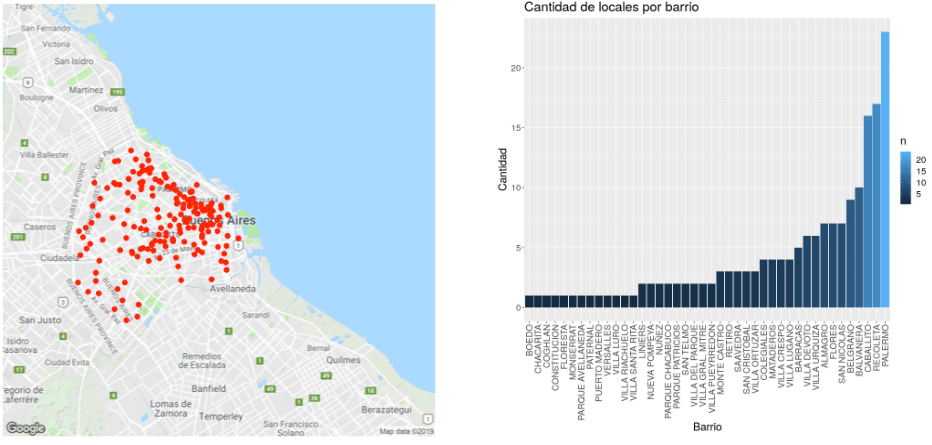
\includegraphics[width=0.9\textwidth]{img/cantLocales_vs_barrio_mapa.png}
}%
\caption{Ubicación de puntos de venta}
\label{ptos_venta}
\end{figure}



Lo que se puede observar de este primer análisis es que los puntos de venta no están repartidos uniformemente y es clara una mayor concentración de puntos de venta hacia la zona del centro norte de la Ciudad, donde se encuentra la mayor densidad poblacional \cite{densidad} y áreas de oficina.\\
Por otro lado en el segundo gráfico de la figura \ref{ptos_venta} se observa una asimetría a izquierda, acumulando 5 barrios del 42 el 44\% del total de las sucursales y solo Palermo representando el 13\% de las mismás.\\
Lo que se busca a continuación es entender cómo es el precio medio de los productos agrupados por barrio, esto ayudará a poder dilucidar si existe alguna correlación entre la cantidad de puntos de ventas en un barrio con su precio promedio.
¿Es necesariamente el barrio con menos cantidad de puntos de ventas el que tiene el precio más alto promedio (por tener una menor cantidad de oferta)?\\
¿O por el contrario el mayor precio se dará en barrios con más cantidad de locales?\\

\newpage

\begin{figure}[h]
\centering
\fbox{
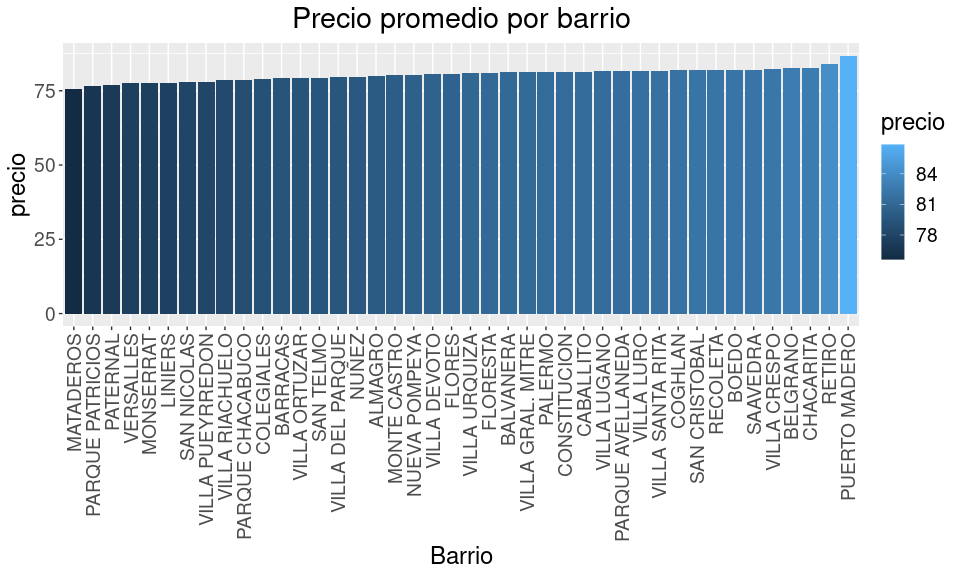
\includegraphics[width=0.9\textwidth]{img/mediaPrecios_xBarrio.png}
}%
\caption{Media de precios}
\label{media_precios}
\end{figure}

Del análisis realizado sobre los distintos barrios de la Ciudad de Buenos Aires se pueden desprender dos conclusiones prematuramente estudiando la figura \ref{media_precios}, una es que si bien algunos barrios han tenido diferencia de precios según el corte donde se tomo la medición, la tendencia en la ventana de tiempo estudiada es siempre al alza. La segunda es que Mataderos, el barrio con el promedio de precios más bajos de entre los 42, tenia muchos más puntos de venta que Puerto Madero, sin embargo este último tiene los mayores precios en promedio de entre todos los barrios porteños. \\


\begin{wrapfigure}{l}{0.4\textwidth}
\centering
\fbox{
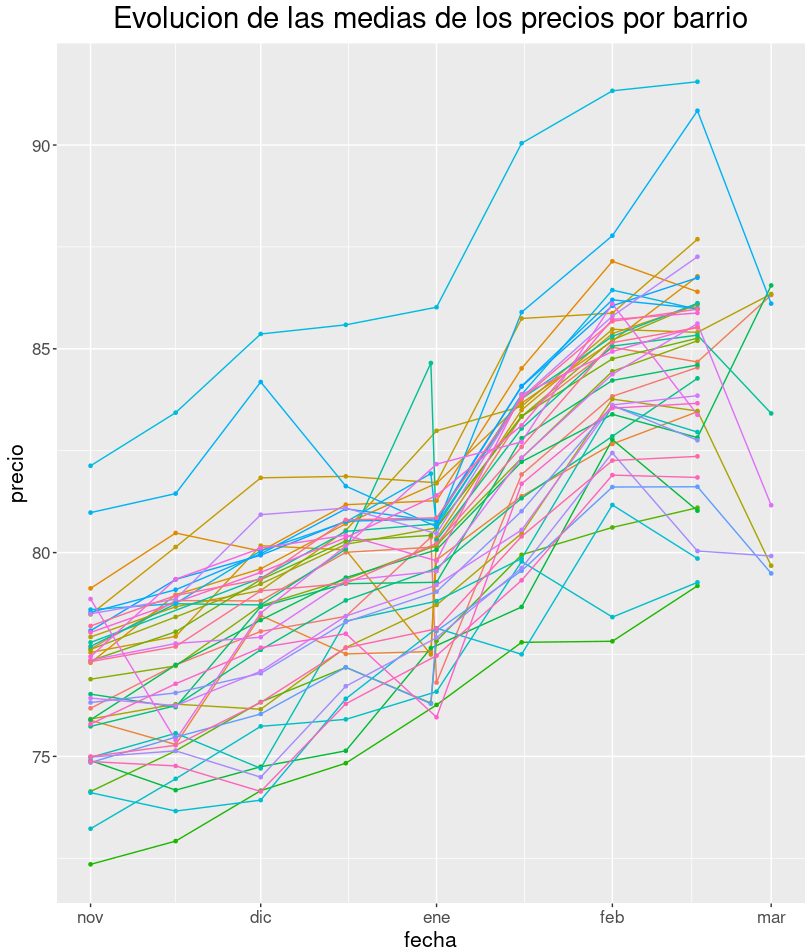
\includegraphics[width=0.35\textwidth]{img/mediaPrecios_agrupados_xBarrio.png}
}%
\caption{Media de precios}
\label{media_precios}
\end{wrapfigure}

Palermo quien ostenta tener el 13\%  de los puntos de venta de la ciudad queda en el puesto 17 de entre los 42 barrios en nivel de precio. Con lo cual hasta ahora no se puede afirmar que la cantidad de sucursales son lo único que influye para determinar el precio promedio de los productos, seguramente el problema incluye más variables que en conjunto determinan el valor de los productos.\\
Lo que si es interesante ver es que no importa el barrio, la tendencia de precios en el periodo estudiado es siempre al alza, como se puede ver en la figura \ref{media_precios} con el consolidado de promedio de precios para todos los barrios de la ciudad.\\


\section{Puntos de venta}

Llega el turno de entender cómo el tipo de punto de venta influye en la distribución de los mismos por la ciudad y en la formación de precios. Para eso, cabe aclarar que se tuvo en cuenta los dos tipos que están representados en el set de datos el de \textbf{Supermercado} y el de \textbf{Hipermercado} siendo este último por lo general de mayor tamaño y contar con más cantidad de productos a la venta. 
Además del tamaño del punto de venta otro estudio que se realizará es el de bandera, cadena o razón social. Cabe destacar que algunas cadenas de supermercado tienen más de una bandera o sub-cadena, tema que se irá ahondando más adelante.\\
Algo que interesa conocer, para iniciar este análisis, es si de los 175 locales la distribución de banderas en dichos locales es uniforme o si hay banderas que tienen predominancia sobre otras.


\begin{figure}[h]
\centering
\fbox{
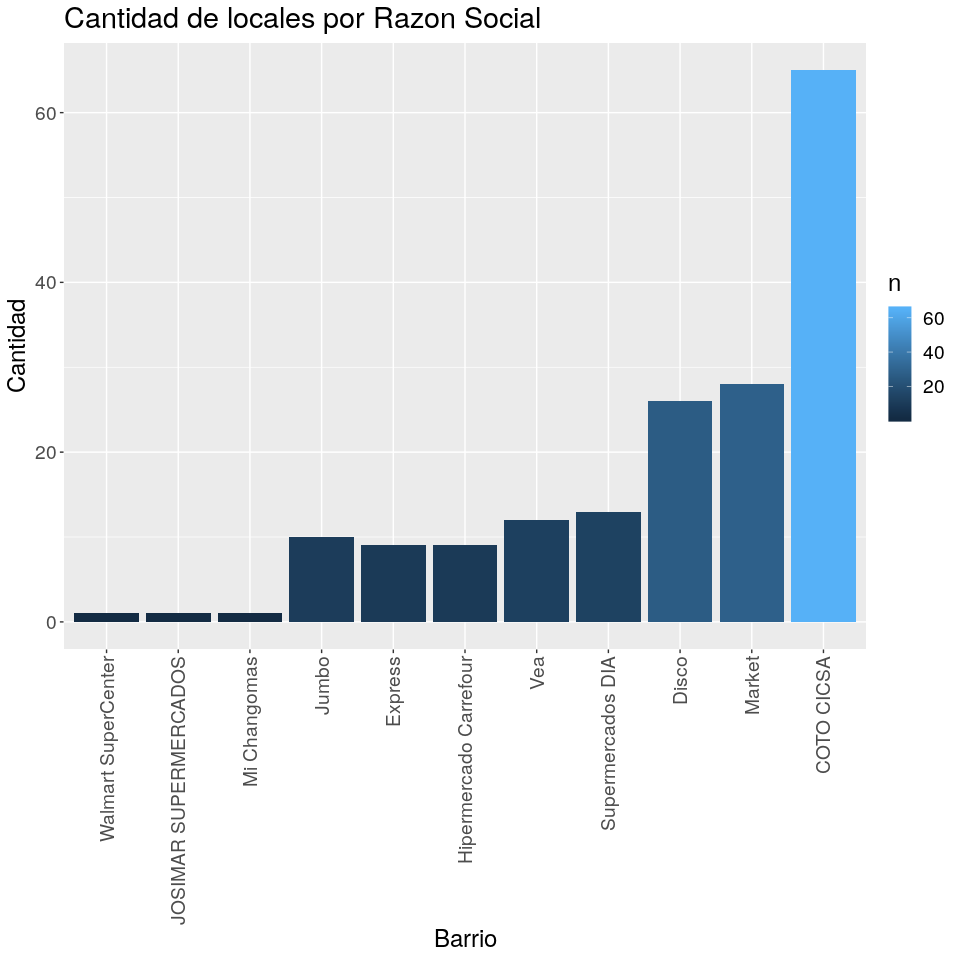
\includegraphics[width=0.9\textwidth]{img/cantLocales_vs_bandera.png}
}%
\caption{Locales por cadena}
\label{Locales_x_cadena}
\end{figure}





Siempre teniendo en cuenta que se están mirando negocios de venta de productos del tipo supermercado o hipermercado, se resalta claramente en la figura \ref{Locales_x_cadena} que en la Ciudad de Buenos Aires, la bandera COTO CICSA tiene una predominancia de casi el 40\% de los locales de venta.\\

Luego de haber tenido este análisis incipiente en la distribución de puntos de venta por las distintas banderas de las empresas, interesa conocer dada una bandera como es la distribución de los precios para todo el periodo estudiado, esto ayudará a entender si existe una bandera con alta predominancia de locales y si son estos los que contienen los precios más altos o más bajos.\\
Se busca entender si existe una bandera formadora de precios, es decir una bandera con fuerte presencia de puntos de venta y precio más elevados que sus competidores.\\




\begin{figure}[h]
\centering
\fbox{
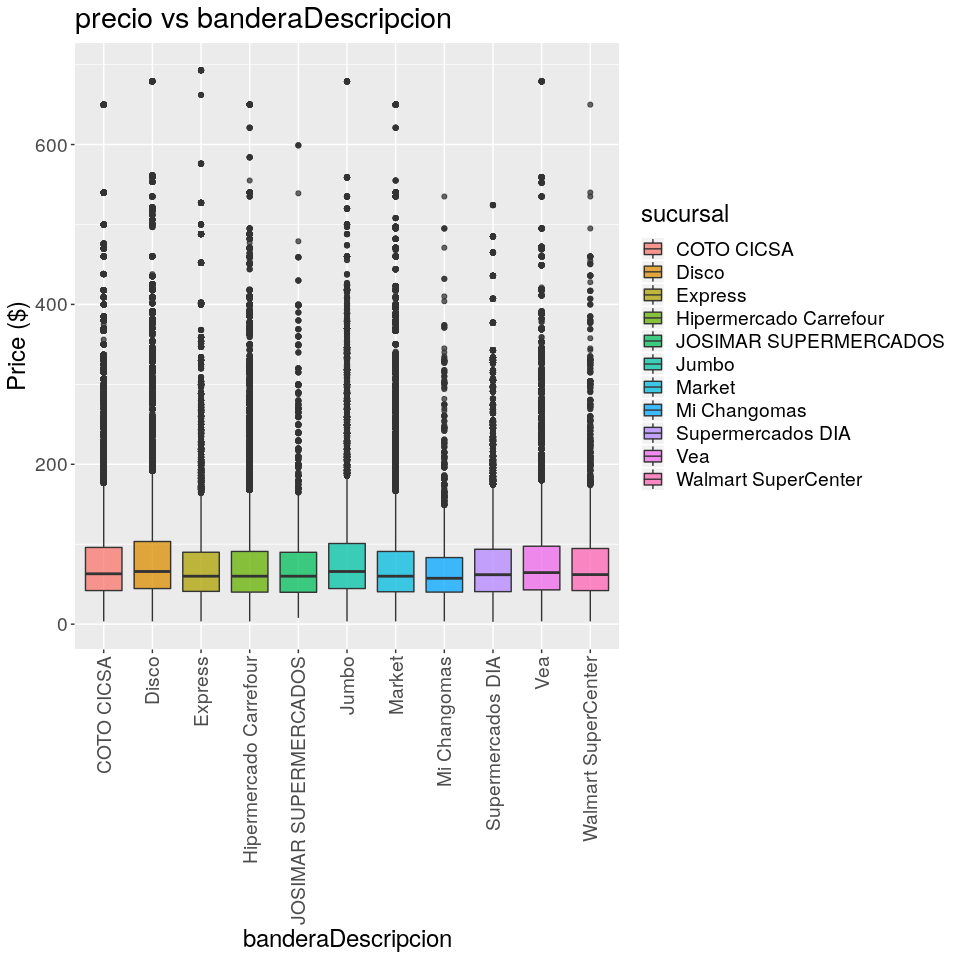
\includegraphics[width=0.4\textwidth]{img/precio_vs_bandera.png}
}%
\hspace{0.25cm}%
\fbox{
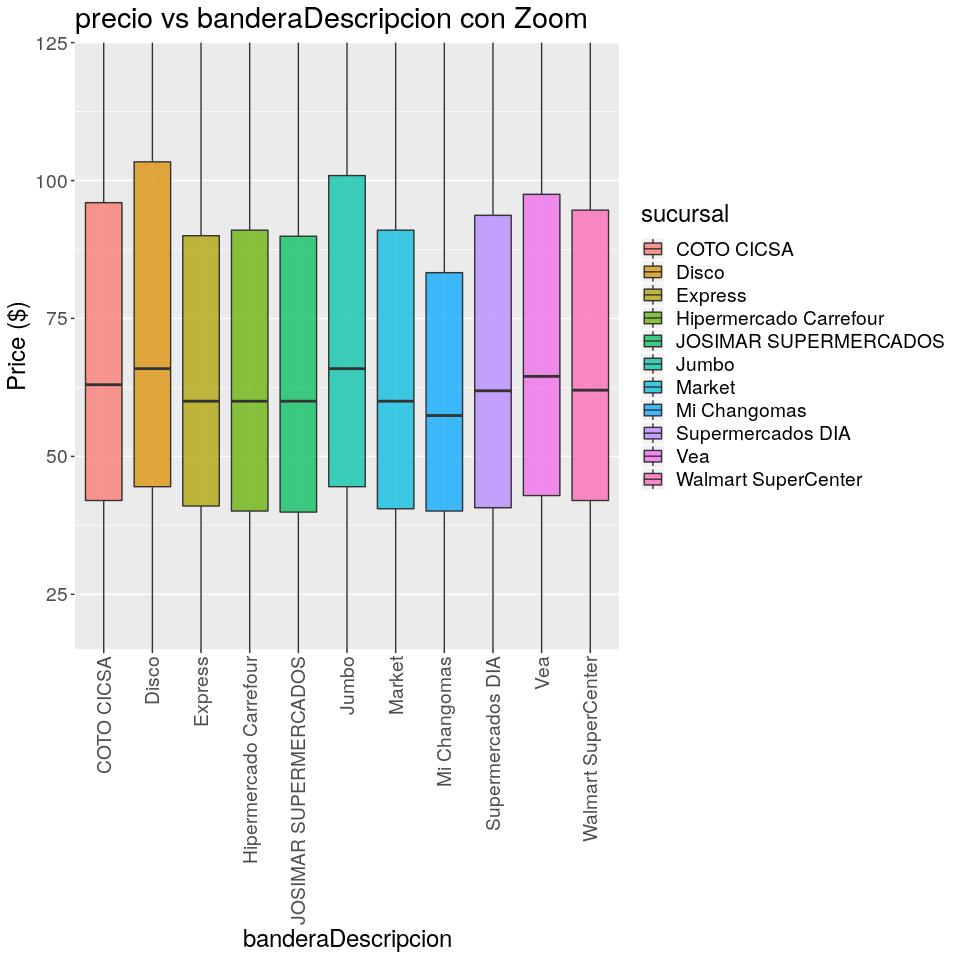
\includegraphics[width=0.4\textwidth]{img/precio_vs_bandera_zoom.png}
}
\caption{Precios vs Banderas}
\label{Precios_vs_Banderas}
\end{figure}


Para hacer este análisis se utilizo BoxPlot, en el gráfico de la izquierda de la figura \ref{Precios_vs_Banderas}, podemos ver como todas las banderas tienen datos de precios muy por arriba del limite superior de las cajas, la gran mayoría entre el rango de los 180 y los 420 PESOS. Sin embargo, lo que es dato es que los precios inferiores son bastante consistente entre las banderas y no se encuentran datos atípicos.\\
En el gráfico de la derecha, lo que se obtiene es un zoom en la zona de las cajas, para entender como es la distribución de los cuantiles y la mediana. Ahí claramente se puede ver que DISCO y JUMBO (ambos de la misma empresa) tienen los precios más altos seguidos por VEA, también del mismo grupo, acaparando entre los tres 48 puntos de venta de los 175 totales, en segundo lugar como grupo está COTO CISCA con 65 puntos de venta de entre las 175.\\
Dado este análisis, se puede concluir que de las 175 sucursales estudiadas dos empresas (COTO y JUMBO-DISCO-VEA) acumulan casi el 65\% de la presencia en el mercado teniendo estos los precios más altos de entre todas las banderas.\\
\newpage
A continuación se realiza un corte cada 15 días para calcular el promedio de precios agrupados por grupo de banderas (en este caso Jumbo, Disco y Vea son agrupados en Jumbo Retail Argentina S.A. ya que pertenecen todos al mismo grupo).

\begin{figure}[h]
\centering
\fbox{
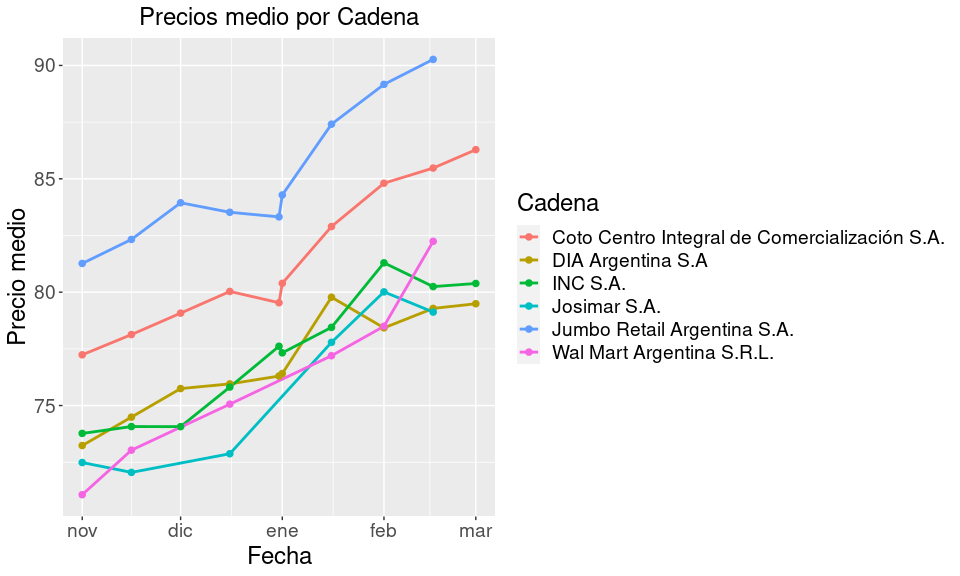
\includegraphics[width=0.45\textwidth]{img/mediaPrecios_xCadena.png}
}%
\hspace{0.25cm}%
\fbox{
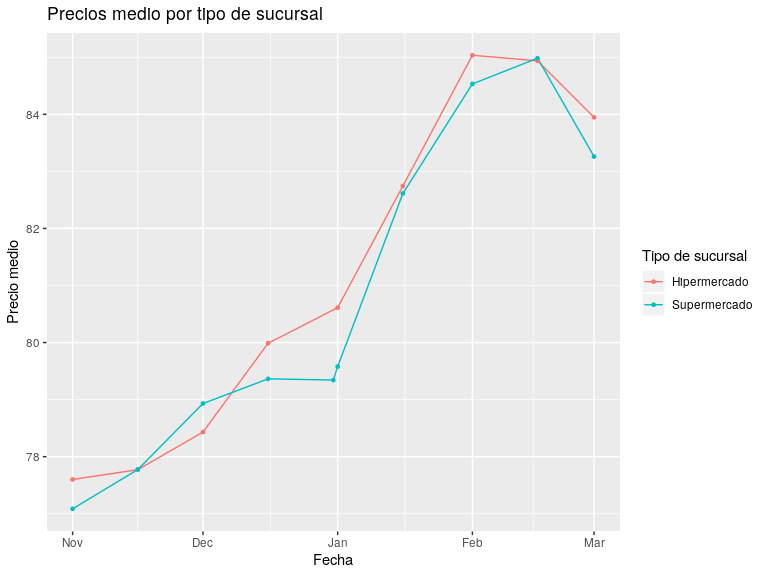
\includegraphics[width=0.45\textwidth]{img/mediaPrecios_vs_tipoLocal.png}
}
\caption{Distribución de precios por tipo bandera y comparativa de promedios cada 15 días}
\label{Distr_comparativa}
\end{figure}


Se puede comprobar en el gráfico izquierdo de la figura \ref{Distr_comparativa}, con un corte promedio cada 15 días, que el conglomerado de Jumbo y Coto siguen una curva muy parecida y claramente tienen los precios promedio más altos y además definen en el tiempo una tendencia al alza.\\
El resto de las banderas, con menor presencia también tienen una tendencia al alza pero con precios promedios menores.\\
En la figura \ref{Distr_comparativa} derecha se observa una comparativa entre todas las banderas diferenciando los Supermercados de los Hipermercados. Si bien, la tendencia y las curvas de evolución de los precios es muy similar, en la mayoría de los cortes los precios promedio en los Hipermercados es superior a los de los Supermercados.\\

\begin{wrapfigure}{r}{0.5\textwidth}
\centering
\fbox{
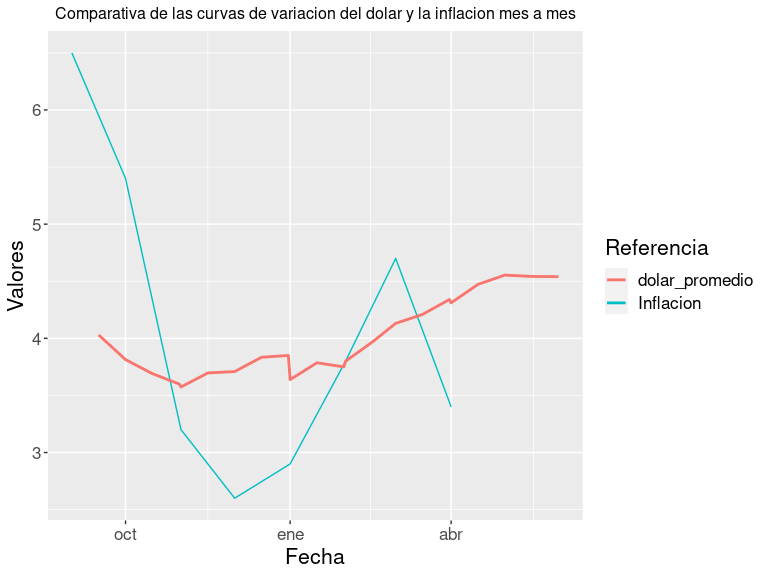
\includegraphics[width=0.42\textwidth]{img/dolar_vs_inflasion.png}
}%
\caption{Dolar vs Inflación}
\label{dolar_vs_inflasion}
\end{wrapfigure}

Como último punto exploratorio se busco entender cúal es la tendencia entre la inflación informada por el INDEC \cite{indec} y el precio del Dolar Norteamericano \cite{cotDolar} promedio compra y venta (se reviso el periodo y el spread entre ambos valores estuvo acotado en todo momento) y se puede comprobar mediante la figura \ref{dolar_vs_inflasion} que el comportamiento de la inflación para este período fue mucho más fluctuante que el precio promedio del dolar con cortes cada 15 días, el cual mostró un comportamiento más parecido a los precios de los productos de góndolas, siempre al alza. Esto podría deberse a que la medición de la inflación que se tomo de referencia es un solo valor mensual que engloba muchos dominios diferentes, los alimentos y productos de este trabajo son uno pero también hay otros rubros como ser servicios, transportes y demás que pueden tener un comportamiento completamente diferente al de los productos estudiados.